\section{Experimental design}
The primary comparison uses a controlled synthetic evidence generator with process, authentication, and network-flow claims, original/derived observations, missing and contradictory fields, and recorded availability minutes. Eight training queues and ten development queues (200 expert top-20 opportunities) supported method development. The frozen development candidate obtained 169/200 Recall@20, 177/200 recoverability, and 73/100 P@10, with no false grouped pairs or mixed groups. It missed the predeclared 170/200 development gate by one incident. A documented subsequent decision permitted evaluation of the unchanged candidate on a new holdout; this was a protocol adjustment, not a passed development gate.

\begin{figure}[ht]
\centering
\includegraphics[width=\linewidth]{fig3}
\caption{Experimental protocol overview: controlled training, development with the missed gate condition, documented authorization, and frozen holdout evaluation. Source/prediction hashes were SHA-256 sealed before private-truth access. No post-result holdout tuning occurred.}
\label{fig:expoverview}
\end{figure}

The holdout used seed 31103, template variant 2, and 15 queues, with 5,018 eligible alerts and 300 expert top-20 opportunities. Baseline and candidate predicted the same alert sets. Source/configuration hashes were frozen; prediction and decision files were SHA-256 sealed before the unchanged evaluator accessed private truth. Each arm was evaluated once. The holdout is within the synthetic generator family and uses a distinct template variant; it is not an operational dataset. Figures~\ref{fig:protocol} and~\ref{fig:devtraj} illustrate the experimental separation and development trajectory.
\begin{figure}[ht]\centering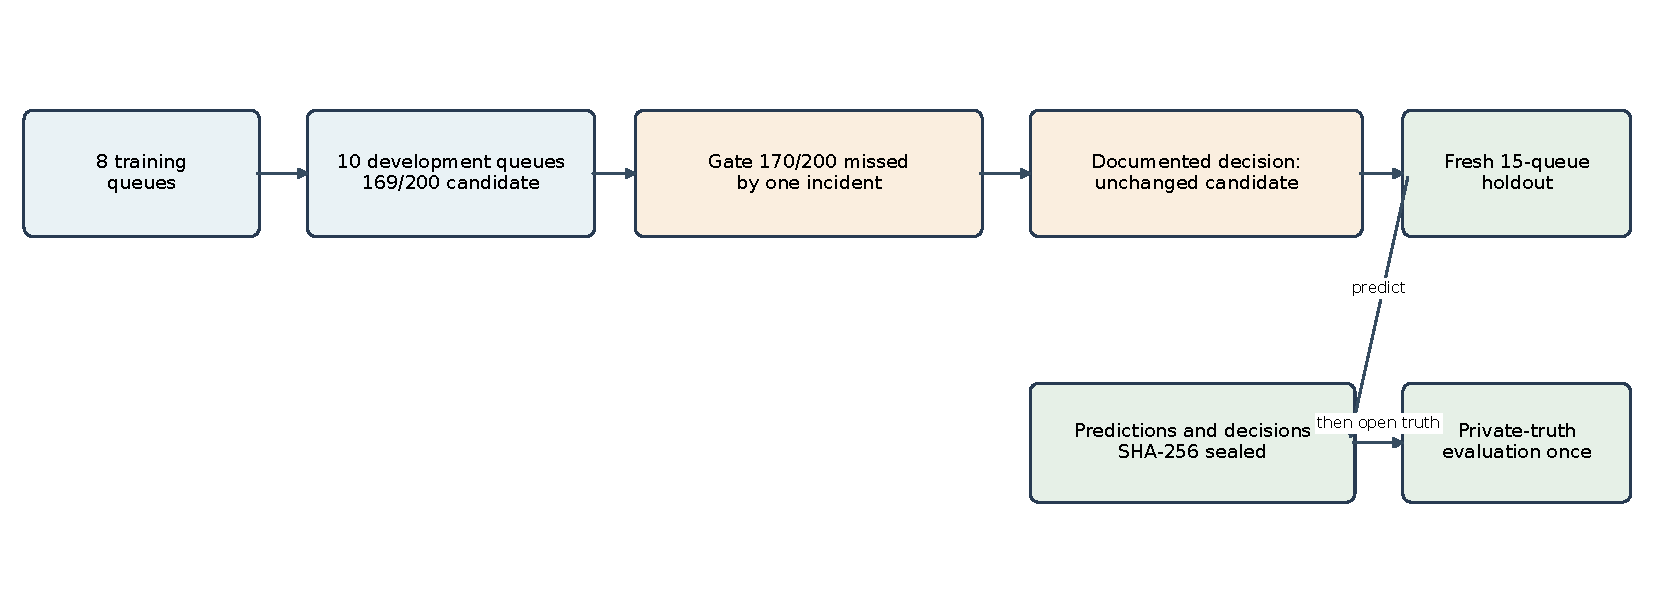
\includegraphics[width=\linewidth]{figures/experimental_protocol.pdf}\caption{Experimental order: training and development, the missed 170/200 development gate, the documented authorization to test the unchanged candidate, a fresh synthetic holdout, SHA-256 sealing, and one subsequent private-truth evaluation. No post-result holdout tuning is represented.}\label{fig:protocol}\end{figure}
\begin{figure}[ht]\centering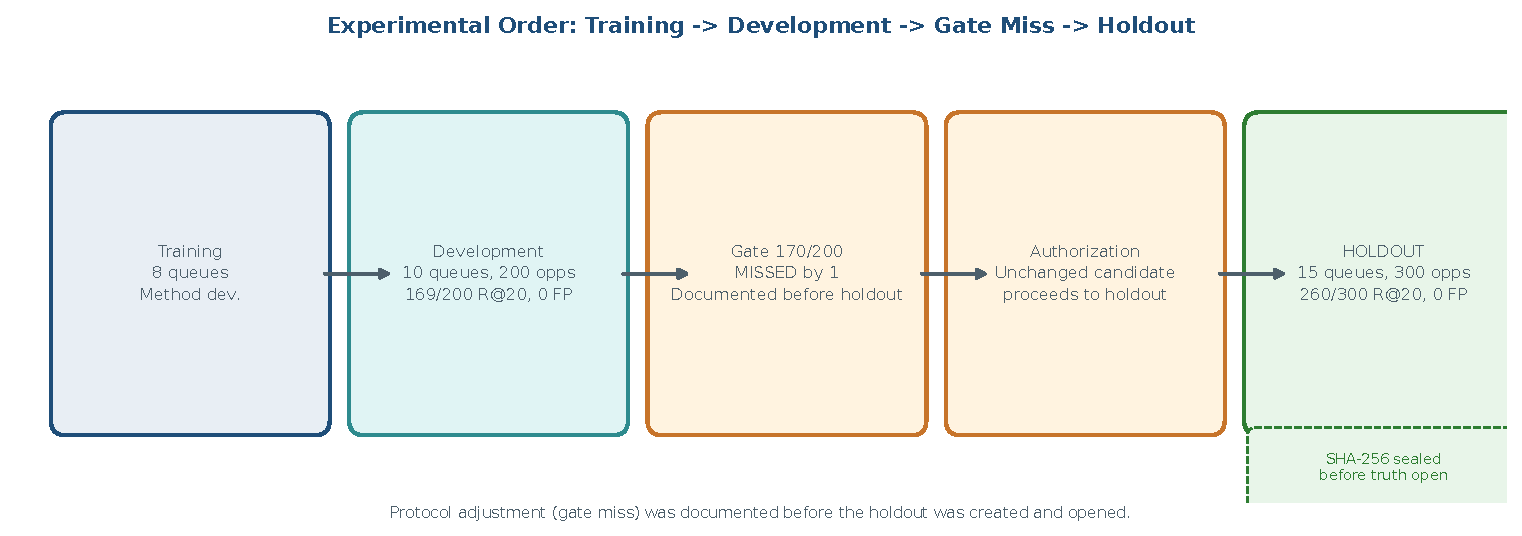
\includegraphics[width=\linewidth]{figures/dev_trajectory.pdf}\caption{Annotated development trajectory from training through holdout. The gate miss and authorization decision are shown explicitly; both occurred before the holdout population was created or any truth label was accessed.}\label{fig:devtraj}\end{figure}

\begin{table}[ht]\centering\small\caption{Distinct research populations. Separate development cohorts in later studies cannot be pooled with the primary holdout.}\label{tab:cohorts}\begin{tabularx}{\linewidth}{@{}p{32mm}p{27mm}Y@{}}\toprule Population & Size & Role and boundary\\\midrule Controlled training & 8 queues & Generator-family method development; private holdout not involved\\ Controlled development & 10 queues; 200 top-20 opportunities & Candidate selection and one-incident gate miss\\ Frozen holdout & 15 queues; 5,018 eligible alerts; 300 top-20 opportunities & Paired baseline/candidate evaluation after prediction seal\\ Later studies & Separate development cohorts, generally 15 queues each & Diagnostic and ranking investigations; no fresh promoted holdout\\ GUIDE inspection & 4,147,992 evidence rows & Schema/readiness audit; no model predictions\\\bottomrule\end{tabularx}\end{table}
